\documentclass[11pt]{article}
\usepackage{theme}
\usepackage{shortcuts}
% Document parameters
% Document title
\title{Assignment 1 (ML for TS) - MVA}
\author{
Darius Dabert \email{darius.dabert@polytechnique.edu} \\ % student 1
Elia El Khoury \email{eliaelkhoury2@gmail.com} % student 2
}

\begin{document}
\maketitle

\section{Introduction}

\paragraph{Objective.} This assignment has three parts: questions about convolutional dictionary learning, spectral features, and a data study using the DTW. 

\paragraph{Warning and advice.} 
\begin{itemize}
    \item Use code from the tutorials as well as from other sources. Do not code yourself well-known procedures (e.g., cross-validation or k-means); use an existing implementation. 
    \item The associated notebook contains some hints and several helper functions.
    \item Be concise. Answers are not expected to be longer than a few sentences (omitting calculations).
\end{itemize}



\paragraph{Instructions.}
\begin{itemize}
    \item Fill in your names and emails at the top of the document.
    \item Hand in your report (one per pair of students) by Tuesday 28\textsuperscript{th} October 23:59 PM.
    \item Rename your report and notebook as follows:\\ \texttt{FirstnameLastname1\_FirstnameLastname2.pdf} and\\ \texttt{FirstnameLastname1\_FirstnameLastname2.ipynb}.\\
    For instance, \texttt{LaurentOudre\_CharlesTruong.pdf}.
    \item Upload your report (PDF file) and notebook (IPYNB file) using this link: \footnotesize{LINK}.
\end{itemize}


\section{Convolution dictionary learning}

\begin{exercise}
Consider the following Lasso regression:
\begin{equation}\label{eq:lasso}
    \min_{\beta\in\RR^p} \frac{1}{2}\norm{y-X\beta}^2_2 \quad + \quad \lambda \norm{\beta}_1
\end{equation}
where $y\in\RR^n$ is the response vector, $X\in\RR^{n\times p}$ the design matrix, $\beta\in\RR^p$ the vector of regressors and $\lambda>0$ the smoothing parameter.

Show that there exists $\lambda_{\max}$ such that the minimizer of~\eqref{eq:lasso} is $\mathbf{0}_p$ (a $p$-dimensional vector of zeros) for any $\lambda > \lambda_{\max}$. 
\end{exercise}

\begin{solution} 

Let

\[
\lambda_{\text{max}} = \max_j \left| \sum_{i=1}^{n} y_i x_{ij} \right|
\]

\[
\forall j, \quad \lambda_{\text{max}} |\beta_j| \geq  \beta_j \left| \sum_{i=1}^{n} y_i x_{ij} \right|
\]

\[
 \lambda_{\text{max}} \|\beta\|_1 \geq  \sum_{j=1}^{p} |\beta_j| \lambda_{\text{max}}  \geq  y^T X \beta 
\]

\[
\lambda_{\text{max}} \|\beta\|_1 + \frac{1}{2} \beta^T X^T X \beta - y^T X \beta \geq 0
\]

since $X^T X$ is symetric semi-definite positive. 

and
\[
f(\beta) \geq f(0)
\quad \Rightarrow \quad \arg \min f(\beta) = 0^p \quad \text{si} \quad \lambda > \lambda_{\text{max}}
\]

\[
\boxed{\lambda_{\text{max}} = \max_j \left| \sum_{i=1}^{n} y_i x_{ij} \right| =  \|X^Ty \|_{\infty} }
\]


\end{solution}


\begin{exercise}
For a univariate signal $\mathbf{x}\in\mathbb{R}^n$ with $n$ samples, the convolutional dictionary learning task amounts to solving the following optimization problem:

\begin{equation}
\min_{(\mathbf{d}_k)_k, (\mathbf{z}_k)_k \\ \norm{\mathbf{d}_k}_2^2\leq 1} \quad\norm{\mathbf{x} - \sum_{k=1}^K \mathbf{z}_k * \mathbf{d}_k }^2_2 \quad + \quad\lambda \sum_{k=1}^K \norm{\mathbf{z}_k}_1
\end{equation}

where $\mathbf{d}_k\in\mathbb{R}^L$ are the $K$ dictionary atoms (patterns), $\mathbf{z}_k\in\mathbb{R}^{N-L+1}$ are activations signals, and $\lambda>0$ is the smoothing parameter.

Show that
\begin{itemize}
    \item for a fixed dictionary, the sparse coding problem is a lasso regression (explicit the response vector and the design matrix);
    \item for a fixed dictionary, there exists $\lambda_{\max}$ (which depends on the dictionary) such that the sparse codes are only 0 for any $\lambda > \lambda_{\max}$. 
\end{itemize}
\end{exercise}

\begin{solution}  % ANSWER HERE

\begin{itemize}
    \item Let's start by writing the vector $\sum_{k=1}^{K} \mathbf{z}_k * \mathbf{d}_k$ as $\mathbf{D}\mathbf{Z}$ where $\mathbf{D} \in \mathbb{R}^{N \times KN}$ and $\mathbf{Z} \in \mathbb{R}^{KN}$.
    
    We have, for element $i \in [1,N]$:
    \[
    \left( \sum_{k=1}^{K} \mathbf{z}_k * \mathbf{d}_k \right)_i = \sum_{k=1}^{K} \sum_{j=1}^{N} \mathbf{z}_k(j) \, \mathbf{d}_k(i-j) \tag{$\star$}
    \]
    
    such that $\mathbf{z}_k(j) =
    \begin{cases}
    (\mathbf{z}_k)_j & \text{if } 1 \leq j \leq N-L+1 \\
    0 & \text{otherwise}
    \end{cases}$
    
    and $\mathbf{d}_k(i-j) =
    \begin{cases}
    (\mathbf{d}_k)_{i-j} & \text{if } 1 \leq i-j \leq L \\
    0 & \text{otherwise}
    \end{cases}$
    
    And, for element $i \in [1,N]$:
    \[
    \left(\mathbf{DZ} \right)_i = \sum_{j=1}^{KN} \mathbf{D}_{ij}\mathbf{Z}_j \tag{$\star$}
    \]
    
    This gives us $\mathbf{Z} = \left(\mathbf{z}_1, 0, \dots, 0, \mathbf{z}_2, 0, \dots, 0, \dots, \mathbf{z}_K, 0, \dots, 0\right) \in \mathbb{R}^{KN}.$
    
    And $\mathbf{D} = (\mathbf{D}_1, \mathbf{D}_2, \dots, \mathbf{D}_K)$ where for each $k \in [1,K]:$
    \[
    (\mathbf{D}_k)_{ij} = \mathbf{d}_k(i-j)
    \]
    
    With these notations, the sparse coding problem is in fact a lasso regression.

    \item Using Q.1 we have $\boxed{\lambda_{\max} = \norm{\mathbf{D}^T\mathbf{x}}_\infty}$
    
\end{itemize}


\end{solution}

\section{Spectral feature}

Let $X_n$ ($n=0,\dots, N-1)$ be a weakly stationary random process with zero mean and autocovariance function $\gamma(\tau):= \mathbb{E}(X_n X_{n+\tau})$.
Assume the autocovariances are absolutely summable, \ie $\sum_{\tau\in\mathbb{Z}} |\gamma(\tau)| < \infty$, and square summable, \ie $\sum_{\tau\in\mathbb{Z}} \gamma^2(\tau) < \infty$.
Denote the sampling frequency by $f_s$, meaning that the index $n$ corresponds to the time $n / f_s$. For simplicity, let $N$ be even.


The \textit{power spectrum} $S$ of the stationary random process $X$ is defined as the Fourier transform of the autocovariance function:
\begin{equation}
    S(f) := \sum_{\tau=-\infty}^{+\infty}\gamma(\tau)e^{-2\pi f\tau/f_s}.
\end{equation}
The power spectrum describes the distribution of power in the frequency space. 
Intuitively, large values of $S(f)$ indicate that the signal contains a sine wave at the frequency $f$.
There are many estimation procedures to determine this important quantity, which can then be used in a machine-learning pipeline.
In the following, we discuss the large sample properties of simple estimation procedures and the relationship between the power spectrum and the autocorrelation.

(Hint: use the many results on quadratic forms of Gaussian random variables to limit the number of calculations.)

\begin{exercise}
In this question, let $X_n$ ($n=0,\dots,N-1)$ be a Gaussian white noise.

\begin{itemize}
    \item Calculate the associated autocovariance function and power spectrum. (By analogy with the light, this process is called ``white'' because of the particular form of its power spectrum.)
\end{itemize}

\end{exercise}

\begin{solution}
Soit $\tau \in \mathbb{Z}$

\[
\gamma(\tau) = \mathbb{E}\left(X_n X_{n+\tau}\right) = \begin{cases}
\sigma^2 & \text{si } \tau = 0 \\
0 & \text{sinon}
\end{cases}
\]

\[
S(f) = \sigma^2
\]

\end{solution}


\begin{exercise}
A natural estimator for the autocorrelation function is the sample autocovariance
\begin{equation}
    \hat{\gamma}(\tau) := (1/N) \sum_{n=0}^{N-\tau-1} X_n X_{n+\tau}
\end{equation}
for $\tau=0,1,\dots,N-1$ and $\hat{\gamma}(\tau):=\hat{\gamma}(-\tau)$ for $\tau=-(N-1),\dots,-1$.
\begin{itemize}
    \item Show that $\hat{\gamma}(\tau)$ is a biased estimator of $\gamma(\tau)$ but asymptotically unbiased.
    What would be a simple way to de-bias this estimator?
\end{itemize}

\end{exercise}

\begin{solution}

\[
\mathbb{E}\left[\hat{\gamma}(\tau)\right] = \frac{1}{N} \sum_{n=0}^{N-\tau-1} \mathbb{E}\left(X_n X_{n+\tau}\right)
\]

\[
= \gamma(\tau) \frac{N - \tau}{N}
\]

\[
\overset{N \to \infty}{\longrightarrow} \gamma(\tau)
\]

\[
\hat{\gamma}_{\text{unbiased}}(\tau) = \frac{1}{N-\tau} \sum_{n=0}^{N-\tau-1} X_n X_{n+\tau}
\]

\end{solution}

\begin{exercise}
Define the discrete Fourier transform of the random process $\{X_n\}_n$ by
\begin{equation}
    J(f) := (1/\sqrt{N})\sum_{n=0}^{N-1} X_n e^{-2\pi\iu f n/f_s}
\end{equation}
The \textit{periodogram} is the collection of values $|J(f_0)|^2$, $|J(f_1)|^2$, \dots, $|J(f_{N/2})|^2$ where $f_k = f_s k/N$.
(They can be efficiently computed using the Fast Fourier Transform.)
\begin{itemize}
    \item Write $|J(f_k)|^2$ as a function of the sample autocovariances.
    \item For a frequency $f$, define $f^{(N)}$ the closest Fourier frequency $f_k$ to $f$.
    Show that $|J(f^{(N)})|^2$ is an asymptotically unbiased estimator of $S(f)$ for $f>0$.
\end{itemize}
\end{exercise}

\begin{solution}

Let $f \in [0, N/2]$,
\begin{align*}
| J(f_k) |^2 &= \frac{1}{N} \sum_{n=0}^{N-1} \sum_{p=0}^{N-1} X_n X_p e^{-2i\pi f(n-p)/f_s} \\
&= \frac{1}{N} \sum_{n=0}^{N-1} \sum_{\tau=-(N-1)}^{N-1} X_n X_{n-\tau} e^{-2i\pi f\tau/f_s } \quad (\tau = n - p) \\
&= \frac{1}{N} \sum_{\tau=-(N-1)}^{N-1} \sum_{n=\tau}^{N-1} X_n X_{n-\tau} e^{-2i\pi f\tau/f_s } \\
&= \frac{1}{N} \sum_{\tau=-(N-1)}^{N-1} \left( \sum_{n=0}^{N-\tau-1} X_n X_{n+\tau} \right) e^{-2i\pi f\tau/f_s} \\
&= \sum_{\tau=-(N-1)}^{N-1} \hat{\gamma}^{(N)}(\tau) e^{-2i\pi f\tau/f_s }
\end{align*}

Now, as 

\[
f^{(N)} \xrightarrow{N \to \infty} f:
\]

\[
\mathbb{E} [\hat{\gamma}^{(N)}(\tau)] \xrightarrow{N \to \infty} \gamma(\tau)
\]
and
\[
\mathbb{E} \left[ \hat{\gamma}^{(N)}(\tau) e^{-2i\pi(f\tau/f_s)} \right]^2 \leq |\gamma(\tau)|^2
\]

Thus:
\[
\mathbb{E} \left( | J(f^N) |^2 \right) \xrightarrow{N \to \infty} S(f)
\]
    
\end{solution}

\begin{exercise}\label{ex:wn-exp}
    In this question, let $X_n$ ($n=0,\dots,N-1)$ be a Gaussian white noise with variance $\sigma^2=1$ and set the sampling frequency to $f_s=1$ Hz
    \begin{itemize}
        \item For $N\in\{200, 500, 1000\}$, compute the \textit{sample autocovariances} ($\hat{\gamma}(\tau)$ vs $\tau$) for 100 simulations of $X$.
        Plot the average value as well as the average $\pm$, the standard deviation.
        What do you observe?
        \item For $N\in\{200, 500, 1000\}$, compute the \textit{periodogram} ($|J(f_k)|^2$ vs $f_k$) for 100 simulations of $X$.
        Plot the average value as well as the average $\pm$, the standard deviation.
        What do you observe?
    \end{itemize}
    Add your plots to Figure~\ref{fig:wn-exp}.
    
\begin{figure}
    \centering
    \begin{minipage}[t]{0.3\textwidth}
    \centerline{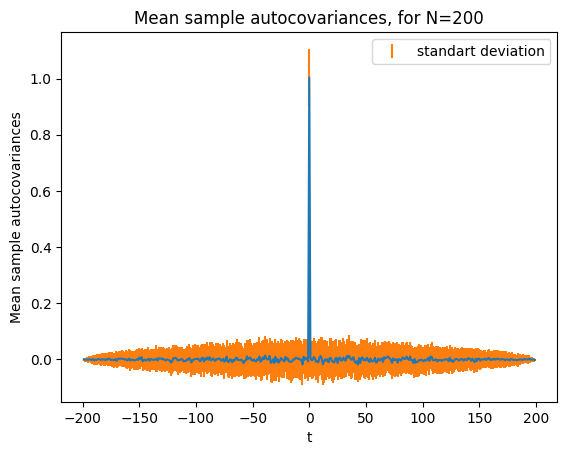
\includegraphics[width=\textwidth]{autocov200}}
    \centerline{Autocovariance ($N=200$)}
    \end{minipage}
    \begin{minipage}[t]{0.3\textwidth}
    \centerline{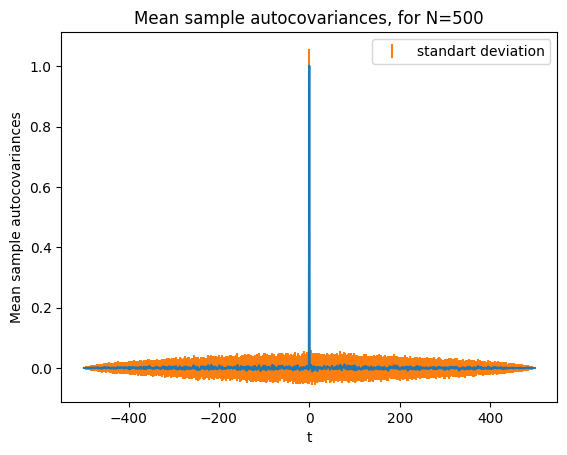
\includegraphics[width=\textwidth]{autocov500}}
    \centerline{Autocovariance ($N=500$)}
    \end{minipage}
    \begin{minipage}[t]{0.3\textwidth}
    \centerline{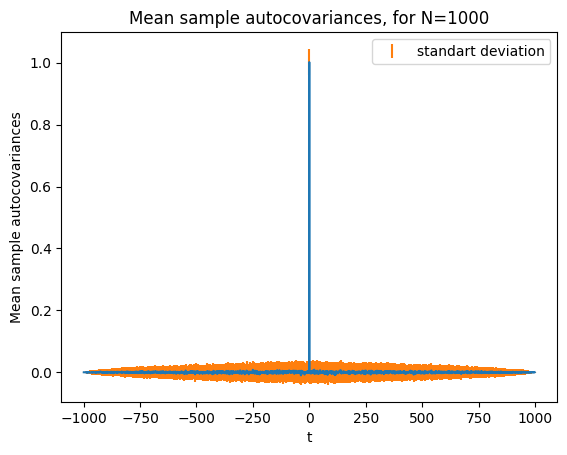
\includegraphics[width=\textwidth]{autocov1000}}
    \centerline{Autocovariance ($N=1000$)}
    \end{minipage}
    \vskip1em
    \begin{minipage}[t]{0.3\textwidth}
    \centerline{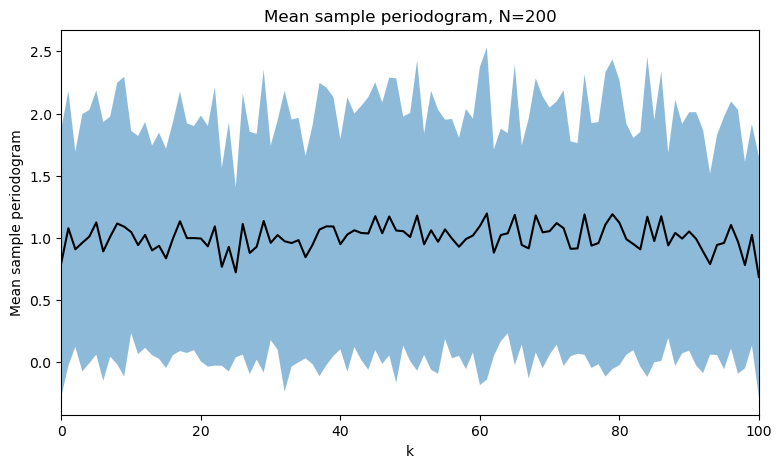
\includegraphics[width=\textwidth]{periodogram200}}
    \centerline{Periodogram ($N=200$)}
    \end{minipage}
    \begin{minipage}[t]{0.3\textwidth}
    \centerline{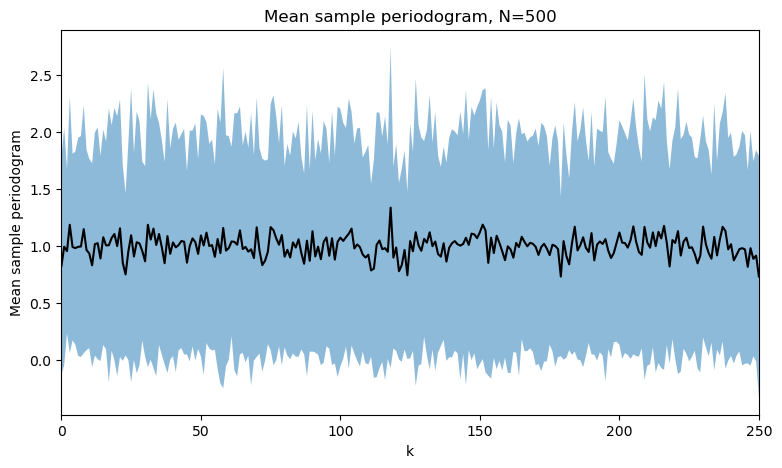
\includegraphics[width=\textwidth]{periodogram500}}
    \centerline{Periodogram ($N=500$)}
    \end{minipage}
    \begin{minipage}[t]{0.3\textwidth}
    \centerline{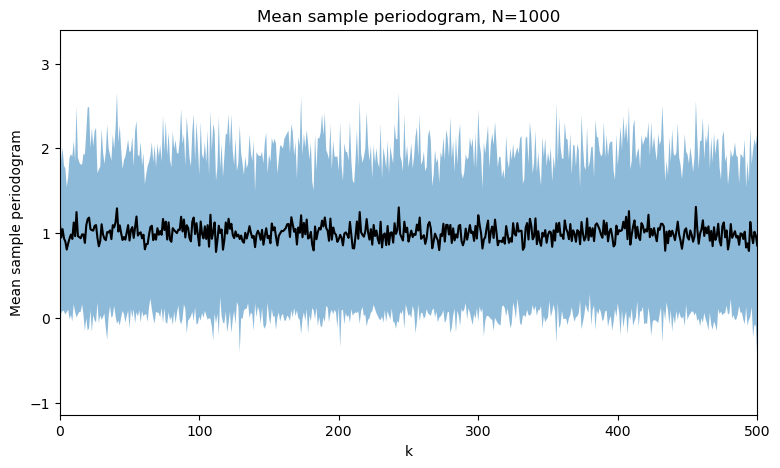
\includegraphics[width=\textwidth]{periodogram1000}}
    \centerline{Periodogram ($N=1000$)}
    \end{minipage}
    \vskip1em
    \caption{Autocovariances and periodograms of a Gaussian white noise (see Question~\ref{ex:wn-exp}).}
    \label{fig:wn-exp}
\end{figure}

\end{exercise}

\begin{solution}
\textbf{Autocovariance:} At $\tau = 0$, the average sample covariance equals the standard deviation, while for $\tau \neq 0$, it approaches 0. The standard deviation decreases with more generations, and the sample covariance seems to tend to 0 for $\tau \neq 0$, consistent with $\hat{\gamma}(\tau)$ being an asymptotically unbiased estimator of $\gamma(\tau)$.

\textbf{Periodogram:} The periodogram shows random, unstable behavior without a clear trend, and its variance does not decrease as the number of samples increases.

    
\end{solution}

\begin{exercise}
    We want to show that the estimator $\hat{\gamma}(\tau)$ is consistent, \ie it converges in probability when the number $N$ of samples grows to $\infty$ to the true value ${\gamma}(\tau)$.
    In this question, assume that $X$ is a wide-sense stationary \textit{Gaussian} process.
    \begin{itemize}
        \item Show that for $\tau>0$ 
    \begin{equation}
       \text{var}(\hat{\gamma}(\tau)) = (1/N) \sum_{n=-(N-\tau-1)}^{n=N-\tau-1} \left(1 - \frac{\tau + |n|}{N}\right) \left[\gamma^2(n) + \gamma(n-\tau)\gamma(n+\tau)\right].
    \end{equation}
    (Hint: if $\{Y_1, Y_2, Y_3, Y_4\}$ are four centered jointly Gaussian variables, then $\mathbb{E}[Y_1 Y_2 Y_3 Y_4] = \mathbb{E}[Y_1 Y_2]\mathbb{E}[Y_3 Y_4] + \mathbb{E}[Y_1 Y_3]\mathbb{E}[Y_2 Y_4] + \mathbb{E}[Y_1 Y_4]\mathbb{E}[Y_2 Y_3]$.) 
    \item Conclude that $\hat{\gamma}(\tau)$ is consistent.
    \end{itemize}
\end{exercise}

\begin{solution}

Let $\tau > 0$.

\[
\text{Var}(\hat{\gamma}(\tau)) = \text{Cov}(\hat{\gamma}(\tau), \hat{\gamma}(\tau))
\]

\[
= \frac{1}{N^2} \sum_{m=0}^{N-\tau-1} \sum_{p=0}^{N-\tau-1} \text{Cov}(X_m X_{m+\tau}, X_p X_{p+\tau})
\]

\[
= \frac{1}{N^2} \sum_{m=0}^{N-\tau-1} \sum_{p=0}^{N-\tau-1} \big[ \mathbb{E}(X_m X_{m+\tau} X_p X_{p+\tau}) - \mathbb{E}(X_m X_{m+\tau}) \mathbb{E}(X_p X_{p+\tau}) \big]
\]

\[
= \frac{1}{N^2} \sum_{m=0}^{N-\tau-1} \sum_{p=0}^{N-\tau-1} \big[ \mathbb{E}(X_m X_p) \mathbb{E}(X_{m+\tau} X_{p+\tau}) + \mathbb{E}(X_m X_{p+\tau}) \mathbb{E}(X_{m+\tau} X_p) - \mathbb{E}(X_m X_{m+\tau}) \mathbb{E}(X_p X_{p+\tau}) \big]
\]

\[
= \frac{1}{N^2} \sum_{m=0}^{N-\tau-1} \sum_{p=0}^{N-\tau-1} \big[ \gamma(m-p)^2 + \gamma(m-p-\tau)\gamma(m-p+\tau) \big]
\]

Let $k = m - p$:

\[
= \frac{1}{N^2} \sum_{m=0}^{N-\tau-1} \sum_{k=-(N-\tau-1)}^{N-\tau-1} \gamma(k)^2 + \gamma(k-\tau)\gamma(k+\tau)
\]

\[
= \frac{1}{N} \sum_{k=-(N-\tau-1)}^{N-\tau-1} \left( \gamma(k)^2 + \gamma(k-\tau) \gamma(k+\tau) \right) \left( 1 - \frac{\tau + |k|}{N} \right)
\]

Since 
\[
\sum_{t \in \mathbb{Z}} \gamma(t)^2 < \infty
\]

\[
\text{Var}(\hat{\gamma}(\tau)) \leq \frac{1}{N} \left( \sum_{k \in \mathbb{Z}} \gamma(k)^2 + \sum_{k \in \mathbb{Z}} \gamma(k - \tau) \gamma(k + \tau) \right)
\]

\[
\leq \frac{2}{N} \sum_{k \in \mathbb{Z}} \gamma(k)^2 \rightarrow 0 \quad \text{as} \quad N \rightarrow \infty
\]

The last inequality and convergence of the second sum in ensured by Cauchy-Schwartz inequality.

With Chebyshev's inequality, we conclude that:

\[
\hat{\gamma}(\tau) \xrightarrow{P} \gamma(\tau) \quad \text{as} \quad N \rightarrow \infty
\]
    
\end{solution}

Contrary to the correlogram, the periodogram is not consistent.
It is one of the most well-known estimators that is asymptotically unbiased but not consistent.
In the following question, this is proven for Gaussian white noise, but this holds for more general stationary processes.
\begin{exercise}
    Assume that $X$ is a Gaussian white noise (variance $\sigma^2$) and let $A(f):=\sum_{n=0}^{N-1} X_n \cos(-2\pi f n/f_s$ and $B(f):=\sum_{n=0}^{N-1} X_n \sin(-2\pi f n/f_s$.
    Observe that $J(f) = (1/N) (A(f) + \iu B(f))$.
    \begin{itemize}
        \item Derive the mean and variance of $A(f)$ and $B(f)$ for $f=f_0, f_1,\dots, f_{N/2}$ where $f_k=f_s k/N$.
        \item What is the distribution of the periodogram values $|J(f_0)|^2$, $|J(f_1)|^2$, \dots, $|J(f_{N/2})|^2$.
        \item What is the variance of the $|J(f_k)|^2$? Conclude that the periodogram is not consistent.
        \item Explain the erratic behavior of the periodogram in Question~\ref{ex:wn-exp} by looking at the covariance between the $|J(f_k)|^2$.
    \end{itemize}
    
\end{exercise}

\begin{solution}

The $X_m$ are independent. Thus,

\[
\mathbb{E}[A(f_l)] = \mathbb{E}[B(f_l)] = 0
\]

\[
\text{Var}(A(f_l)) = \sum_{m=0}^{N-1} \sigma^2 \cos^2(-2 \pi f_l m / f_s) = \sigma^2 \frac{N}{2}
\]

\[
\text{Var}(B(f_l)) = \sum_{m=0}^{N-1} \sigma^2 \sin^2(-2 \pi f_l m / f_s) = \sigma^2 \frac{N}{2}
\]

\[
A(f_l) \sim \mathcal{N} \left(0, \frac{\sigma^2 N}{2} \right), \quad B(f_l) \sim \mathcal{N} \left(0, \frac{\sigma^2 N}{2} \right)
\]

\[
\mathbb{E} \left[ | I(f_l) |^2 \right] = \frac{4}{N} \left[ A^2(f_l) + B^2(f_l) \right]
\]

And 

\[
\frac{A^2(f_l)}{\sigma^2 \frac{N}{2}} \sim \chi^2(1), \quad \frac{B^2(f_l)}{\sigma^2 \frac{N}{2}} \sim \chi^2(1)
\]

Thus,

\[
2 \frac{|I(f_l)|^2}{\sigma^2} \sim \chi^2(2)
\]

\[
\text{Var} \left[ \mathbb{E} \left( | I(f_l) |^2 \right) \right] = \frac{\sigma^4}{4} \text{Var} \left( 2 \frac{|I(f_l)|^2}{\sigma^2} \right)
\]

\[
= \sigma^4
\]

\[
\mathbb{E}\left( \left| J(f_k) \right|^2 \left| J(f_\ell) \right|^2 \right)
= \frac{1}{N^2} \sum_{n=0}^{N-1}  \sum_{m=0}^{N-1} \sum_{p=0}^{N-1}  \sum_{q=0}^{N-1} \mathbb{E}\left( X_n X_{m} X_p X_{q} \right) 
e^{-2 i \pi  \frac{(k(n-p) + \ell(m-q))}{N}f_s} 
\]

\[
= \frac{1}{N^2} \sum_{n=0}^{N-1}  \sum_{m=0}^{N-1} \sum_{p=0}^{N-1}  \sum_{q=0}^{N-1}  \left( \mathbb{E}(X_n X_{m}) \mathbb{E}(X_p X_{q}) 
+ \mathbb{E}(X_n X_p) \mathbb{E}(X_{m} X_{q}) - \mathbb{E}(X_n X_{q}) \mathbb{E}(X_{m} X_p) \right) 
e^{-2 i \pi  \frac{(k(n-p) + \ell(m-q))}{N}f_s} 
\]

\[
= \sigma^4 +  \frac{1}{N^2} \sum_{n=0}^{N-1} \sum_{p=0}^{N-1} \sigma^4  e^{-2 i \pi  \frac{(k+\ell)(n-p)}{N}f_s} 
+ \frac{1}{N^2} \sum_{n=0}^{N-1} \sum_{m=0}^{N-1} \sigma^4  e^{-2 i \pi  \frac{(k-\ell)(n-m)}{N}f_s} \]

\[= \left\{
\begin{array}{ll}
2\sigma^4 & \text{if } k = \ell \\
\sigma^4 & \text{if } k \neq \ell
\end{array}
\right.
\]

Thus, 
\[
\text{cov} \left( \left| J(f_k) \right|^2 \left| J(f_\ell) \right|^2 \right) 
= \left\{
\begin{array}{ll}
\sigma^4 & \text{if } k = \ell \\
0 & \text{if } k \neq \ell
\end{array}
\right.
\]

If k in different from l, there is no correlation between the terms of the periodogram, thus the erratic behavior.
    
\end{solution}

\begin{exercise}\label{q:barlett}
    As seen in the previous question, the problem with the periodogram is the fact that its variance does not decrease with the sample size.
    A simple procedure to obtain a consistent estimate is to divide the signal into $K$ sections of equal durations, compute a periodogram on each section, and average them.
    Provided the sections are independent, this has the effect of dividing the variance by $K$. 
    This procedure is known as Bartlett's procedure.
    \begin{itemize}
        \item Rerun the experiment of Question~\ref{ex:wn-exp}, but replace the periodogram by Barlett's estimate (set $K=5$). What do you observe?
    \end{itemize}
    Add your plots to Figure~\ref{fig:barlett}.
\end{exercise}

\begin{solution}
    
\begin{figure}
    \centering
    \begin{minipage}[t]{0.3\textwidth}
    \centerline{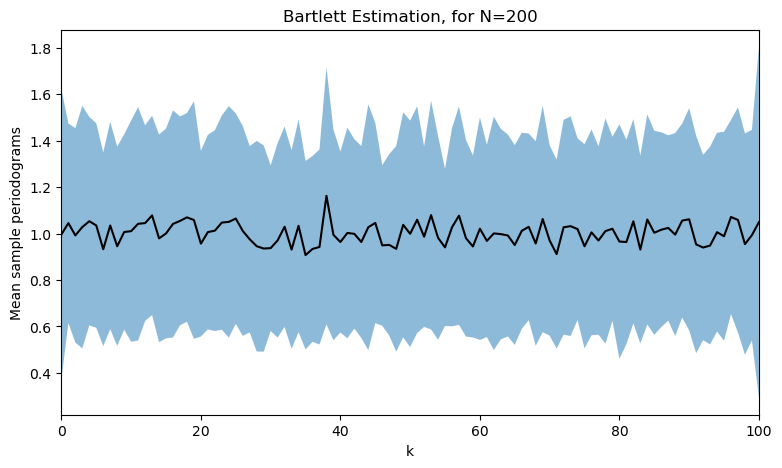
\includegraphics[width=\textwidth]{Barlett200}}
    \centerline{Periodogram ($N=200$)}
    \end{minipage}
    \begin{minipage}[t]{0.3\textwidth}
    \centerline{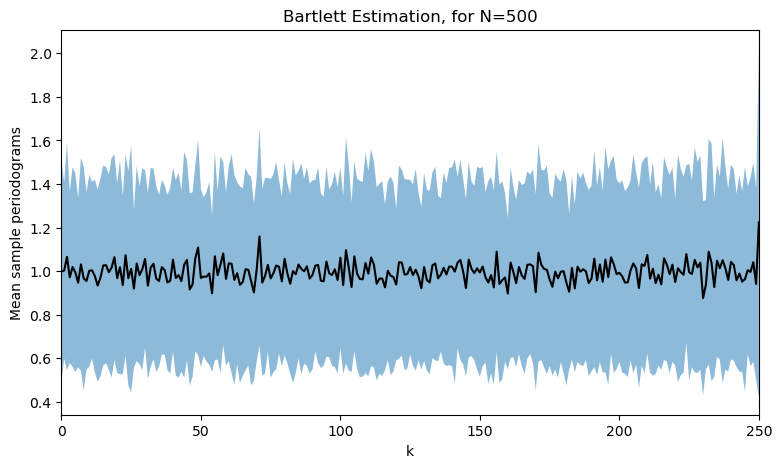
\includegraphics[width=\textwidth]{Barlett500}}
    \centerline{Periodogram ($N=500$)}
    \end{minipage}
    \begin{minipage}[t]{0.3\textwidth}
    \centerline{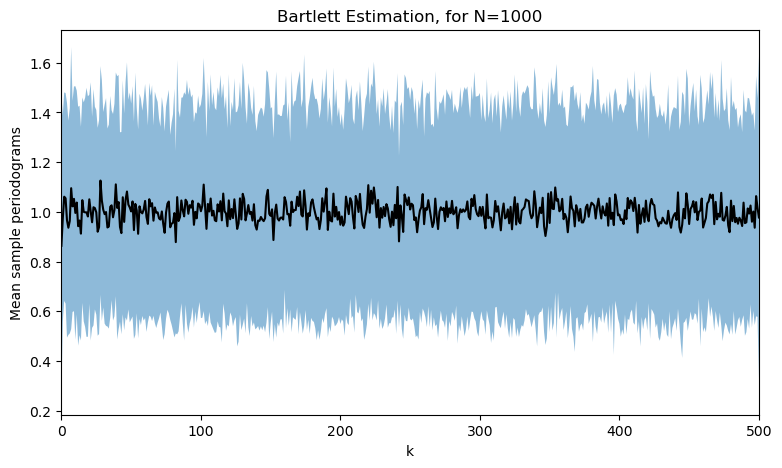
\includegraphics[width=\textwidth]{Barlett1000}}
    \centerline{Periodogram ($N=1000$)}
    \end{minipage}
    \vskip1em
    \caption{Barlett's periodograms of a Gaussian white noise (see Question~\ref{q:barlett}).}
    \label{fig:barlett}
\end{figure}

We observe that compare to Question 6, the standard deviation with this method is smaller, which is in accordance with the principle of the method that divides the variance by a factor 5 and the the standard deviation by a factor $\sqrt{5}$.

\end{solution}
\section{Data study}

\subsection{General information}

\paragraph{Context.}
The study of human gait is a central problem in medical research with far-reaching consequences in the public health domain. This complex mechanism can be altered by a wide range of pathologies (such as Parkinson's disease, arthritis, stroke,\ldots), often resulting in a significant loss of autonomy and an increased risk of falls. Understanding the influence of such medical disorders on a subject's gait would greatly facilitate early detection and prevention of those possibly harmful situations. To address these issues, clinical and bio-mechanical researchers have worked to objectively quantify gait characteristics.

Among the gait features that have proved their relevance in a medical context, several are linked to the notion of step (step duration, variation in step length, etc.), which can be seen as the core atom of the locomotion process. Many algorithms have, therefore, been developed to automatically (or semi-automatically) detect gait events (such as heel-strikes, heel-off, etc.) from accelerometer and gyrometer signals.

\paragraph{Data.}
Data are described in the associated notebook.

\subsection{Step classification with the dynamic time warping (DTW) distance}

\paragraph{Task.} The objective is to classify footsteps and then walk signals between healthy and non-healthy.

\paragraph{Performance metric.} The performance of this binary classification task is measured by the F-score.


\begin{exercise}
Combine the DTW and a k-neighbors classifier to classify each step. Find the optimal number of neighbors with 5-fold cross-validation and report the optimal number of neighbors and the associated F-score. Comment briefly.
\end{exercise}

\begin{solution}

The model is trained using 5-fold cross-validation, with the optimal number of neighbors determined to be 5.
For label 1, the F-score achieved is 0.87 on the training set, while it drops to 0.45 on the test set.
For label 0, the F-score achieved is 0.88 on the training set, while it drops to 0.09 on the test set.


\end{solution}

\newpage
\begin{exercise}\label{q:class-errors}
Display on Figure~\ref{fig:class-errors} a badly classified step from each class (healthy/non-healthy).
\end{exercise}

\begin{solution}
\begin{figure}
    \centering
    \begin{minipage}[t]{\textwidth}
    \centerline{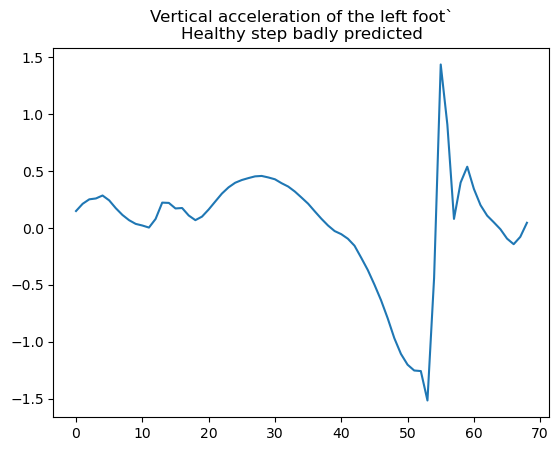
\includegraphics[width=0.6\textwidth]{badly_healthy}}
    \centerline{Badly classified healthy step}
    \end{minipage}
    \vskip1em
    \begin{minipage}[t]{\textwidth}
    \centerline{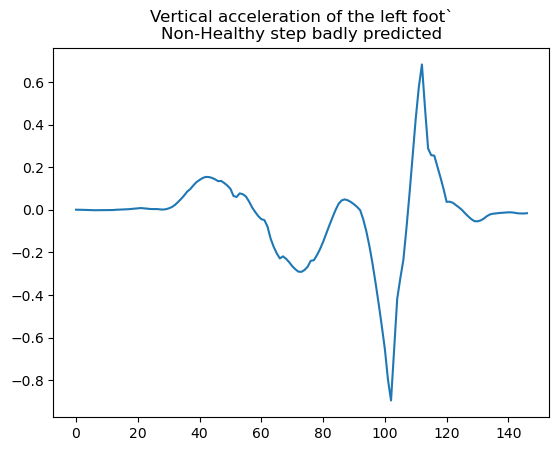
\includegraphics[width=0.6\textwidth]{badly-non-healthy}}
    \centerline{Badly classified non-healthy step}
    \end{minipage}
    \vskip1em
    \caption{Examples of badly classified steps (see Question~\ref{q:class-errors}).}
    \label{fig:class-errors}
\end{figure}
\end{solution}


\end{document}
